%
% Lista de requerimientos funcionales,
% Capítulo de análisis y diseño de api web.
% Proyecto Lovelace
%

\subsubsection{Funcionales}

% Estos son los requerimientos que el analista «deduce» de su plática con el
% cliente. Teóricamente antes de estos tendrían que ir lo de «alto nivel»,
% en donde se exprese directamente las palabras del cliente, pero como eso
% pasó en mi mente, o no pasó en absoluto, van directamente los de bajo
% nivel.
% Requerimientos de bajo nivel:

\requerimiento[rq_api:actores]{API}
{Sobre los actores del sistema}
{
  La aplicación debe contemplar las acciones de tres tipos de actores: un
  \textit{visitante}, que representa a los posibles usuarios que visitan la
  página de promoción del sistema; un \textit{usuario}, que utiliza la interfaz
  web del servicio de tokenización; un \textit{administrador}, que representa a
  la entidad (empresa u organización) que ofrece el servicio de tokenización
  (ver regla de negocio \hipervinculo{rn:servicio_tokenizacion}).

  \subrequerimiento[rq_api:cambios_de_actores]
  {Flujos de actores en la aplicación}
  {
    En la figura \ref{estados_actores} se muestra un diagrama de estados con
    la relación de los actores con la aplicación. Las transiciones representan
    los casos de uso que hacen cambiar al tipo de actor.

    Al abrir la aplicación toda persona es un \textit{visitante}. Los
    \textit{usuarios} y los \textit{administradores} necesitan iniciar sesión
    para ser identificados como tal por el sistema. Un \textit{visitante} puede
    pasar a ser actor al registrarse en el sistema.

    Este requerimiento está relacionado con las reestricciones impuestas por los
    requerimientos \hipervinculo{rq_api:registro_de_actores} y
    \hipervinculo{rq_api:identificacion_de_actores}.
  }
}

% TODO:
% Poner numeración a los casos de uso de las transiciones.
% Cambiar nombre de caso de uso de registro de usarios.
% Arreglar etiqueta de estado «por identificar».

\begin{figure}
  \begin{center}
    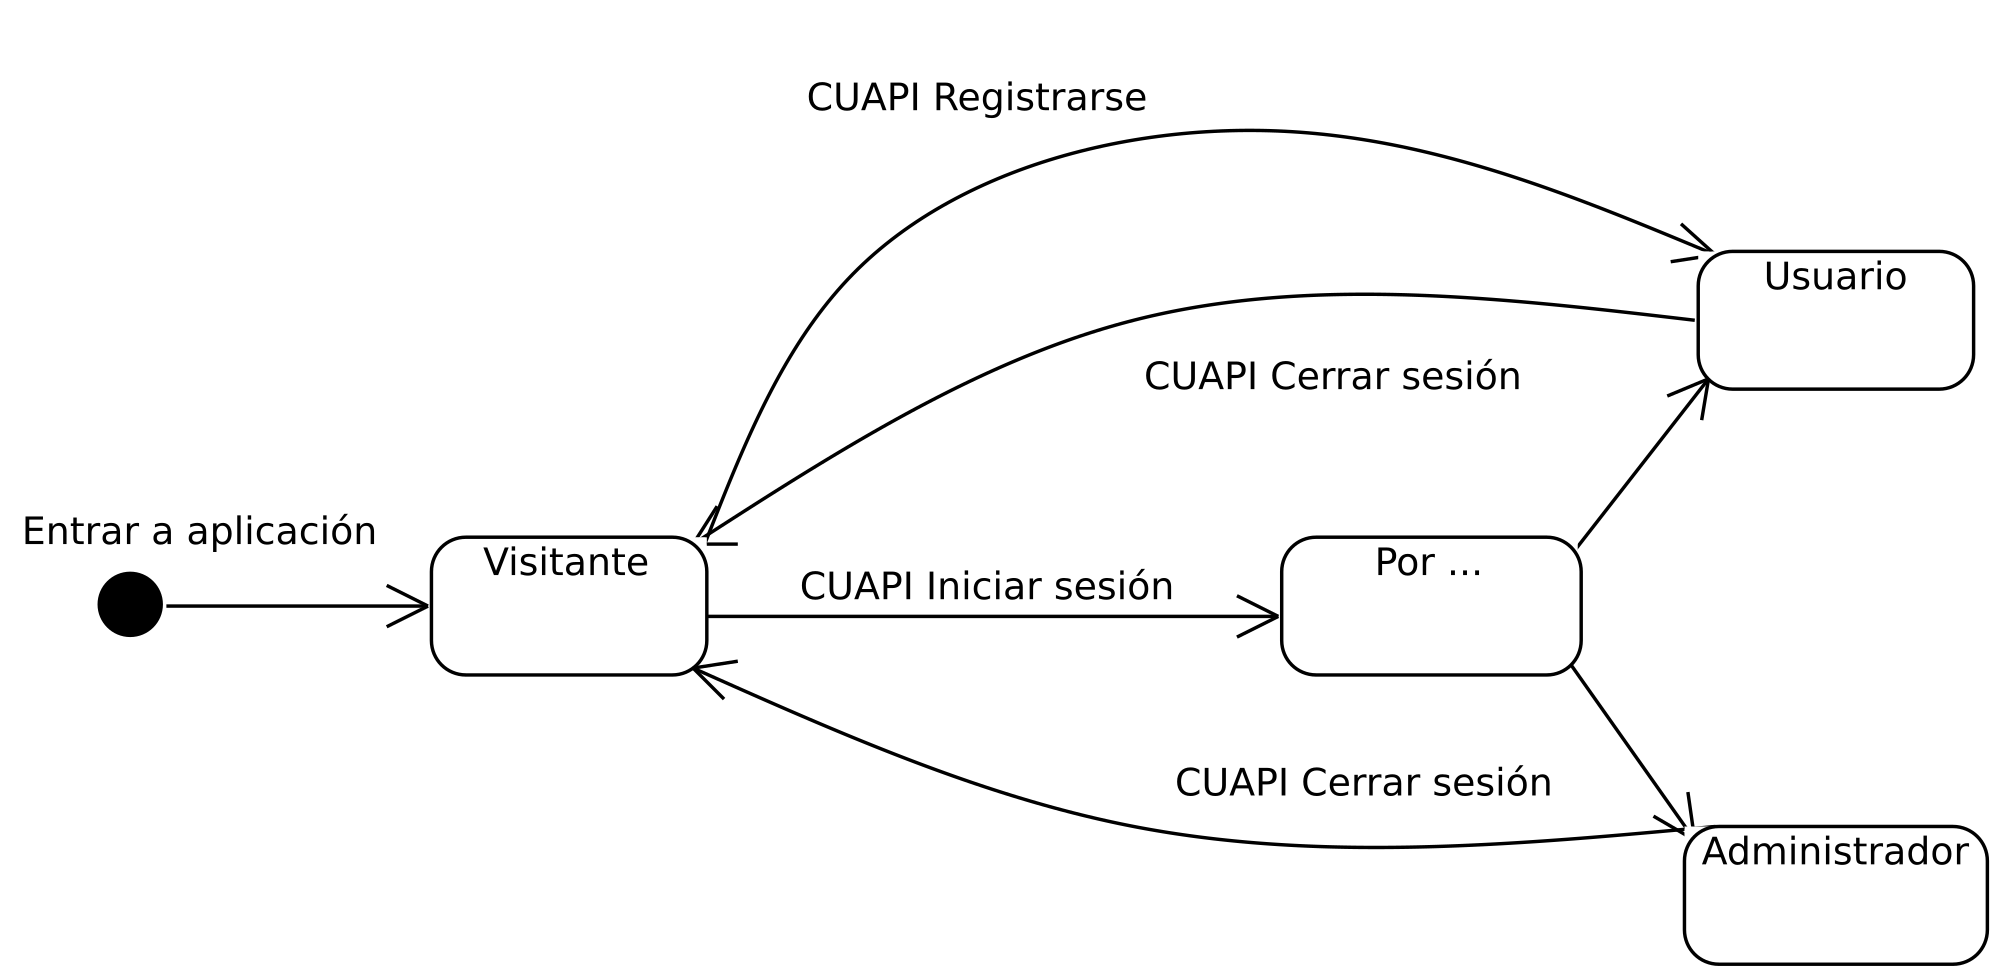
\includegraphics[width=0.8\linewidth]{diagramas/flujo_de_actores.png}
    \caption{Diagrama de estados de actores.}
    \label{estados_actores}
  \end{center}
\end{figure}

% Depende de rq_api:actores
\requerimiento[rq_api:interfaces_de_usuario]{API}
{Sobre las interfaces gráficas del sistema}
{
  La aplicación web debe contar con las interfaces especificadas en los
  siguientes subrequerimientos.

  \subrequerimiento[rq_api:sitio_publico]
  {Sitio público de aplicación}
  {
    Estas páginas deben ser accesibles para los tres actores definidos en
    \hipervinculo{rq_api:actores}.

    \subsubrequerimiento[rq_api:interfaz_inicio]
    {Interfaz de inicio de sitio público}
    {
      Página que debe promocionar el servicio de tokenización. Debe de explicar
      qué es la tokenización y qué es lo que hace el servicio ofrecido. Esta
      interfaz se muestra en \hipervinculo{iu:inicio}.
    }

    \subsubrequerimiento[rq_api:interfaz_documentacion]
    {Interfaz de documentación}
    {
      Página que debe explicar cómo utilizar la \gls{gl:api} web del
      servicio de tokenización. Esta interfaz se muestra en
      \hipervinculo{iu:documentacion}.
    }

    \subsubrequerimiento[rq_api:interfaz_inicio_de_sesion]
    {Interfaz de inicio de sesión}
    {
      Formulario para que los administradores o usuarios inicien sesión en el
      sistema. Esta interfaz se muestra en \hipervinculo{iu:iniciar_sesion}.
    }

    \subsubrequerimiento[rq_api:interfaz_registro_de_usuarios]
    {Interfaz de registro de usuarios}
    {
       Formulario que permite que un visitante se registre como usuario.
       Esta interfaz se muestra en \hipervinculo{iu:registrar_usuario}.
    }
  }

  \subrequerimiento[rq_api:administracion_de_tokens]
  {Sitio de administración de tokens}
  {
    Estas páginas deben ser accesibles solamente a los usuarios
    (\hipervinculo{rq_api:actores}).

    % TODO: ¿Qué hace esta interfaz?
    \subsubrequerimiento[rq_api:interfaz_inicio_usuario]
    {Interfaz de inicio de usuarios}
    {
       Página de bienvenida de un actor tipo usuario. Esta interfaz se
       muestra en \hipervinculo{iu:inicio_usuario}.
    }
  }

  \subrequerimiento[rq_api:administracion_de_usuarios]
  {Sitio de administración general}
  {
    Estas páginas deben ser accesibles solamente a los administradores
    (\hipervinculo{rq_api:actores}).

    % TODO: ¿Qué hace esta interfaz?
    \subsubrequerimiento[rq_api:interfaz_inicio_administrador]
    {Interfaz de inicio de administradores}
    {
      Página de bienvenida de un actor tipo administrador. Esta interfaz se
      muestra en \hipervinculo{iu:inicio_administrador}.
    }
  }
}

\requerimiento[rq_api:identificacion_de_actores]{API}
{Sobre la identificación de los actores}
{
  Para ser vistos como usuarios o administradores, los actores deben
  pasar por un proceso de identificación. La identificación es mediante
  un correo electrónico (\hipervinculo{rn:correo_electronico}) y una
  contraseña (\hipervinculo{rn:formato_de_contrasenias}). Esto está relacionado
  con \hipervinculo{rqnf_api:alamcenamiento_de_contrasenias}.
}

\requerimiento[rq_api:registro_de_actores]{API}
{Sobre el registro de usuarios y administradores}
{
  El conjunto de usuarios debe poder crecer desde la aplicación web, esto es,
  se deben poder registrar nuevos usuarios. El conjunto de administradores es
  fijo desde el inicio, esto es, no se pueden registrar más administradores
  desde la aplicación web.
}
